\newpage
\subsection{Caso d'uso UC11: Registrazione Nuova API}
\label{UC11}
\begin{figure}[ht]
	\centering
	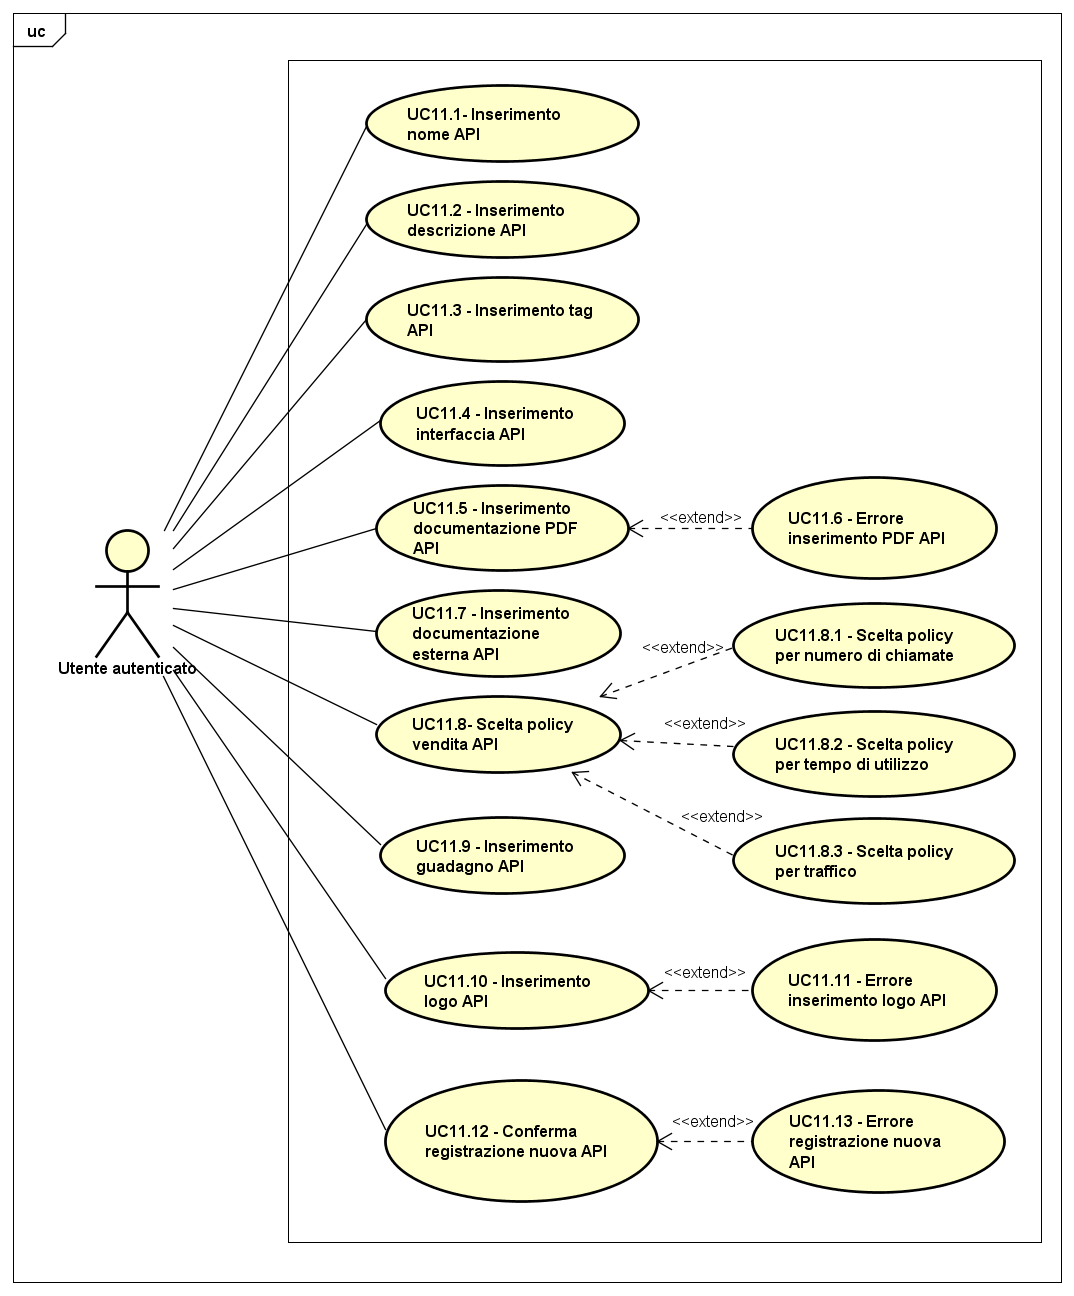
\includegraphics[scale=0.45]{UML/UC11.png}
	\caption{Caso d'uso UC11: Registrazione Nuova API}
\end{figure}

\renewcommand*{\arraystretch}{1.6}
\begin{longtable}{ l | p{11cm}}
	\hline
	\rowcolor{Gray}
	\multicolumn{2}{c}{Caso d'uso UC11: Registrazione Nuova API} \\
	\hline
	\textbf{Attori} &Utente Autenticato, Amministratore APIMarket, Interfacce API Presente In APIMarket \\
	\textbf{Descrizione} & l'attore registra una propria nuova API \\
	\textbf{Pre-Condizioni} &  l'attore ha scelto di registrare una propria nuova API\\
	\textbf{Post-Condizioni}&l'attore ha registrato una propria nuova API\\
	\textbf{Scenario Principale} & \begin{enumerate*}[label=(\arabic*.),itemjoin={\newline}]
		\item L'attore può inserire la documentazione della propria nuova API (UC11.1)
		\item L'attore può registrare l'interfaccia della propria nuova API (UC11.2)
		\item L'attore può confermare la registrazione della propria nuova API (UC11.3)
	\end{enumerate*}\\
	\textbf{Scenari Alternativi} & \begin{enumerate*}[label=(\arabic*.),itemjoin={\newline}]
		\item l'attore visualizza un errore nella registrazione di una propria nuova API (UC11.4)
	\end{enumerate*}\\
\end{longtable}





